\documentclass[main.tex]{subfiles}
% 标架与参考系
\begin{document}
事件世界含有的是一切可以发生的事件,它只是一个供我们讨论某一具体发生着的物理过程的背景概念。若某物体在某段时间之内发生了运动和形变,它将对应于事件世界里的一块子集。具体地,我们把一个\emph{物体(body)}抽象为一个集合$B$,其元素$X,Y,\cdots\in B$称为\emph{物质点(material points)}。在这里我们只讨论物体的\emph{运动学(kinematics)},后续章节会再赋予物体以质量的概念。

现在我们准确地定义什么叫“在一段时间之内”的运动。我们把$\pazocal{T}$的一个连通子集$\Upsilon\subset\pazocal{T}$称作一个\emph{时间段}。所谓“连通”是指,若$t\in\Upsilon$且$t+s\in\Upsilon$,则$t+r\in\Upsilon,\forall r\in\left[0,t\right]$\footnote{这里我们改用小写字母来表示时刻以符合时刻计算的习惯,但需要注意每一时刻都是一个由同时事件组成的欧几里得空间。}。

以下内容可结合图\ref{fig:III.5.2}来理解。

\begin{figure}[ht]
      \centering
      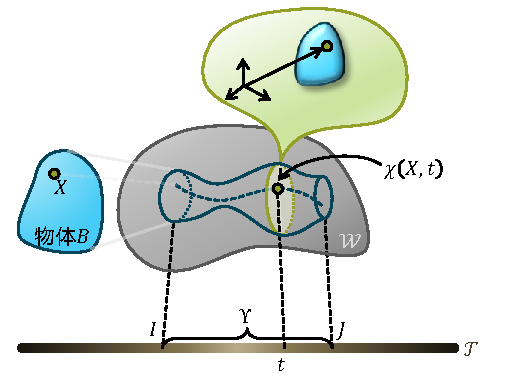
\includegraphics[width=0.5\textwidth]{images/III.5.2.pdf}
      \caption{物体的运动过程、时间线示意图。图中字母符号与文中相同。}
      \label{fig:III.5.2}
\end{figure}

一个物体$B$在时间段$\Upsilon$内的\emph{运动过程(kinematical process)}是一个映射$\chi:B\times\Upsilon\rightarrow\pazocal{W},$
\[\chi\left(X,t\right)\in t,\quad\forall X\in B,\quad\forall t\in\Upsilon\]
再次提醒,上式中的$t$既表示一个时刻又表示这个时刻下的所有同时事件构成的欧几里得空间点集。上述定义实际表达的意思是,想要描述一个由多个物质点构成的物体的运动过程,需且只需说出每个物质点在每个时刻下对应于哪一个物理事件。我们把一个物质点$X\in B$在运动过程$\chi$中的像集
\[\chi\left(X,\Upsilon\right)=\left\{e\in\pazocal{W}|\exists X\in B\forall t\in\Upsilon,e=\chi\left(X,t\right)\right\}\]
(即一个物质点在整个时间段$\Upsilon$内经历的所有事件的集合)称$X$在运动过程$\chi$中的\emph{世界线(worldline)}。

可以留意到,一个物质点在一个运动过程中的世界线上的任意两个不同元素必属于不同时刻。诚然,由运动过程的定义可知,若$t_1,t_2\in\Upsilon$且$t_1\neq t_2$,则物质点$X$在时间段$\Upsilon$内的运动过程$\chi$中的世界线总满足
\[\chi\left(X,t_1\right)\in t_1,\quad\chi\left(X,t_2\right)\in t_2\]
由集合相等的定义,$t_1\neq t_2$决定了$\chi\left(X,t_1\right)\neq\chi\left(X,t_2\right)$。换言之,由$\Upsilon$到$X$在$\chi$中的世界线的映射$t\mapsto\chi\left(X,t\right)$必是单射。

更形象地说,世界线是一条由参数方程定义的曲线\footnote{严格地应该说世界线是一个1维流形。}。一整个物体$B$的运动过程,是$B$的所有物质点形成的\emph{一束}世界线。一个常常默认的公设是\emph{经典时空下的信息守恒,即同一运动过程中的世界线不相交}。这等同于说,一个物体在运动过程中物质点的“数量”守恒\footnote{事实上连续介质物体的物质点数量可能是无穷大的,所以“数量”这一不严谨的说法仅为了辅助理解。}。这是因果决定论所要求的。任一当前时刻的发生的事件必由之前时刻的事件导致(没有“无因之果”),也必导致未来时刻的事件(没有“无果之因”)。

虽然世界线是一条曲线,但它无法直接理解为“质点的轨迹”。因为世界线上不同的事件属于不同时刻,亦属于不同的欧几里得空间的点,无法量度它们之间的距离(只有同时刻的事件之间者能讨论距离)。我们在现实世界中之所以能观测一个质点在两个时刻下的“位移”,必须依赖另一个在这个时间段内也一直出现的另个物体——参照物。就算如此,我们也只能在每一时刻下记录所关心的质点与这一参照物的\emph{相对}距离,得到这个相对距离在两个不同时刻的的差别,来描述这个质点在这两个时刻所规定的时间间隔的标量值的相对位移变化,并进而得到它们的标量相对速率和相对加速率。具体地,我们可以考虑导数
\[\frac{\mathrm{d}}{\mathrm{d}t}\delta\left(\chi\left(X,t\right),\chi\left(Y,t\right)\right)=\lim_{t^\prime\to t}\frac{\delta\left(\chi\left(X,t^\prime\right),\chi\left(Y,t^\prime\right)\right)-\delta\left(\chi\left(X,t\right),\chi\left(Y,t\right)\right)}{t^\prime-t}\]
它是物质点$X$相对于物质点$Y$在时刻$t$下的\emph{相对速率}(标量)。类似地可定义2阶导数为一个标量值的相对加速率。本讲义所考虑的运动过程,任意两个物质点的相对加速率都是连续函数。也就是说,任一运动过程中两物质点的相对距离随时间的变化是2阶光滑的。

现在我们只讨论了两个物质点的相对运动速率和加速率。若要讨论某一个物质点的向量值的位移、速度和加速度等等,就必须在同一欧几里得空间,建立统一的坐标系。这需要引入参考标架的概念。参考标架是在一个观察者的主观视角下的“静止的”3维欧几里得空间\footnote{在经典情况下我们不考虑“空间弯曲”,因此每个观察者视角下的几何空间都是3维欧几里得空间。}。我们习惯说的某物质点的“绝对运动”,事实上是相对于我们视角下的3维欧几里得空间的相对运动。利用上一段介绍的相对运动概念,我们不仅可以把我们所关心的物质点与这个参考标架任一点(物理事件)的相对速率和相对加速率当作这个物质点在这一参考标架下的“绝对”速率和“绝对”加速率,还能利用这一欧几里得空间的平移空间,通过选定原点来实现对这一物质点的向量值位移、速度和加速度的表征。

下面我们严格地给出参考标架的概念。

设一物体$B$在某时间段$\Upsilon$内的运动过程$\chi$中,任意两物质点$X,Y\in B$的距离
\[\delta\left(\chi\left(X,t\right),\chi\left(Y,t\right)\right)\]
保持不依赖时刻$t\in\Upsilon$变化的常数,则称$\chi$是一个\emph{刚体运动过程(rigid body process)}。由相对速率的概念易知,刚体运动过程中任意两物质点相对速率总为零。

若某物体$\mathcal{E}$\emph{永远只能}作刚体运动\footnote{它将会是一个欧几里得空间。},即$\mathcal{E}$在整个时刻空间$\pazocal{T}$内的运动过程$\phi:\mathcal{E}\times\pazocal{T}\rightarrow\pazocal{W}$\emph{总是}一个刚体运动过程——
\[\delta\left(\phi\left(X,t\right),\phi\left(Y,t\right)\right)=d\left(X,Y\right),\quad\forall X,Y\in\mathcal{E},t\in\pazocal{T}\]
其中$d:\mathcal{E}^2\rightarrow\mathbb R$是按照上式定义的$\mathcal{E}$上的一个映射\footnote{我们很快将说明它其实是$\mathcal{E}$上的一个度量。},则称$\mathcal{E}$是一个\emph{刚体系(rigid system)}。上式同时也说明映射$d$的性质沿自$\delta$。因$\delta$是$\pazocal{T}$的每一时刻下的欧几里得度量(见规定D1、D2),故$d$是$\mathcal{E}$上的欧几里得度量,$\left(\mathcal{E},d\right)$由此形成一个欧几里得空间。我们称具有欧几里得空间构造的刚体系$\mathcal{E}$及其某一运动过程$\phi$的组合$\left(\mathcal{E},\phi\right)$为\emph{参考标架(frame of reference)}或简称\emph{标架(frame)};$\mathcal{E}$是这一参考标架的欧几里得空间;$\phi$本身称作\emph{参考运动过程(kinematic process of reference)}。由于可选作参考标架的刚体系$\mathcal{E}$可有不止一个,刚体运动$\phi$也可有不止一种,故参考标架的建立方式也不止一种。参考标架反映的是一名观察者的主观视角或主观选择。

一名观察者在选定了一个参考标架$\left(\mathcal{E},\phi\right)$后,仍然面临着在其欧几里得空间$\mathcal{E}$上建立不同的坐标系的选择。至少要在欧几里得空间$\mathcal{E}$的基本直角坐标系(选定的某原点$O\in\mathcal{E}$和标准基$\left\{\mathbf{\hat{e}}_1,\mathbf{\hat{e}}_2,\mathbf{\hat{e}}_3\right\}$)中,任一时刻$t$的下的事件才对应于一组有序实数三元组$\left(x_1,x_2,x_3\right)\in\mathbb{R}^3$。当然,他也可以在$\mathcal{E}$上建立各种曲线坐标系,同样也能实现任一时刻$t$下使一个事件对应于一组有序实数三元组。在最一般情况下,仅为了这一目的,他完全可以在每一时刻都选一个不同的坐标系。在实际问题中我们选定的坐标系是不依赖时间变化的。严格来说,时刻空间$\pazocal{T}$虽与$\mathbb{R}$同构,但任一时刻$t\in\pazocal{T}$到底对应于$\mathbb{R}$的哪个数值,也仍需在选定某时刻空间的原点$t_0\in\pazocal{T}$并记其为实数$0$后,才能得到确定。我们常常选择$\Upsilon$的边界点作为$t_0$,使$\Upsilon$同构于$\mathbb{R}$上的某连通区间$\left[0,s\right]$。

总而言之,想要使一个物理事件$e\in\pazocal{W}$对应于获得4个实数$\left(t;x_1,x_2,x_3\right)\in\mathbb{R}^{1+3}$的对应,必须具备以下条件:
\begin{itemize}
      \item 事件$e$属于某世界线,也就是说属于某一时间段$\Upsilon\subset\pazocal{T}$中的运动$\chi$;
      \item 已选定某参考标架$\left(\mathcal{E},\phi\right)$;
      \item 已选定起始时刻$t_0\in\pazocal{T}$;
      \item 已选定$\mathcal{E}$下的坐标系
\end{itemize}
\end{document}